% Section 2 of the Part B report: the price of dictatorship (additive valuations).
% Requires \usepackage{wrapfig}.  Proofs: appendix_sd_proofs.tex (app:sd).
% Figure: figures/02_optimal_menu.png (generated by experiments/report_figures.py).

\section{The price of dictatorship}
\label{sec:dictatorship}

Section~\ref{sec:replication} leaves LIP($a^\star$) within about $0.006$ of the best
strategy-proof mechanism. Is the remaining gap due to LIP's particular (linear) price schedule,
or to its dictatorial structure? The paper organises its mechanisms in the nested families
$\mathrm{LIP}\subsetneq\mathrm{IP}\subsetneq\mathrm{SD}\subsetneq\mathrm{SP}$ (linear
increasing-price, increasing-price, swap-dictatorial, all strategy-proof), but bounds only the
two ends. We locate SD exactly.

Like Theorem~1, the best swap-dictatorial mechanism on a type grid is a linear program: the menu
items are the variables, and both incentive and welfare constraints are linear in them. Its value
is exactly $5/6$ on every grid we tried, and the optimal dual uses only the three types
$\{0,\tfrac12,1\}$ and no incentive constraint at all. This pointed to the following short proof.

\begin{theorem}[A]\label{thm:A}
Let $M(x,y)=\lambda A(x)+(1-\lambda)B(y)$, $\lambda\in[0,1]$, where $A$ depends only on agent~1's
report and $B$ only on agent~2's. Then $M$ is at most $5/6$-competitive. In particular this holds
for every swap-dictatorial mechanism, with arbitrary (even agent-specific) menus and lotteries.
\end{theorem}
\begin{proof}
Let $a(x)$ be agent~1's expected share of item~1 minus item~2 under $A(x)$, and $b(y)$ likewise
under $B(y)$; both lie in $[-1,1]$. With additive valuations an allocation with net share $d$
for agent~1 yields welfare $1+(x-y)d$, so $W(x,y)=1+(x-y)[\lambda a(x)+(1-\lambda)b(y)]$. On the four
profiles $(\tfrac12,0),(1,\tfrac12),(0,\tfrac12),(\tfrac12,1)$, each with first-best welfare $\tfrac32$,
the terms of the middle type cancel and
\[
\textstyle\sum W=4+\tfrac12\lambda\,[a(1)-a(0)]+\tfrac12(1-\lambda)\,[b(1)-b(0)]\le5 ,
\]
so some profile has $W\le\tfrac54=\tfrac56\cdot\tfrac32$.
\end{proof}

\begin{wrapfigure}{r}{0.45\linewidth}
\centering
\vspace{-1ex}
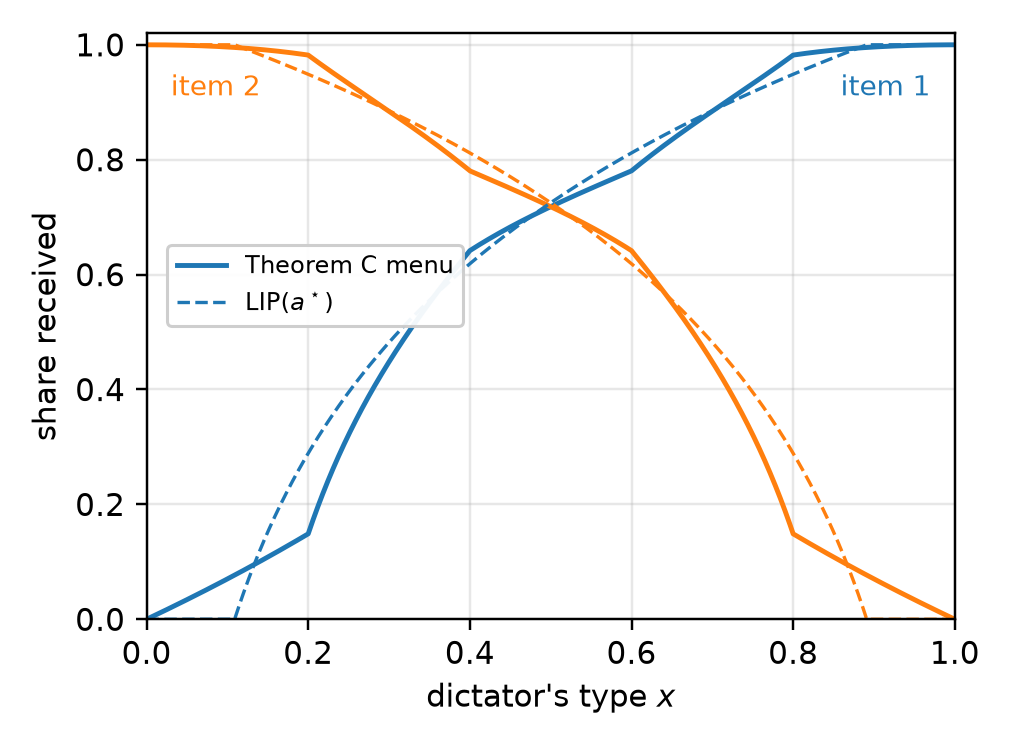
\includegraphics[width=\linewidth]{figures/02_optimal_menu.png}
\caption{What a dictator of type $x$ receives under the Theorem~C menu (solid) and under
LIP($a^\star$) (dashed); blue: item~1, orange: item~2.}
\label{fig:optimal_menu}
\vspace{-2ex}
\end{wrapfigure}

\begin{theorem}[C]\label{thm:C}
The bound is attained: there is a swap-dictatorial mechanism that is exactly $5/6$-competitive.
\end{theorem}
\noindent The construction (Appendix~\ref{app:sd}) reduces a symmetric menu to the dictator's net
share $d(x)=m_1(x)-m_2(x)$. For $x>y$ welfare is $1+\tfrac12(x-y)[d(x)-d(y)]$ against a first best of
$1+(x-y)$, so the mechanism is $5/6$-competitive exactly when
$d(x)-d(y)\ge h(x-y):=\tfrac53-\tfrac{1}{3(x-y)}$, while strategy-proofness only requires $d$ to be
non-decreasing. The steepest admissible increase from $0$ to $x$ is
$D(x)=\max_k\big[\tfrac{5k}{3}-\tfrac{k^2}{3x}\big]$, which reaches exactly $D(1)=2$, the full range
of $d$; the symmetrised $d(x)=\tfrac12[D(x)-D(1-x)]$ is admissible and defines the menu.
Discretising it into 8001 items and evaluating exactly on the continuum gives $0.83328$.

Hence, for two items and additive valuations,
\[
\alpha(\mathrm{LIP}(2))=0.8281\;<\;\alpha(\mathrm{LIP}(a^\star))=0.8294\;<\;\max_{\mathrm{SD}}\alpha=\tfrac56=0.8333\;\le\;\max_{\mathrm{SP}}\alpha\le0.8363 .
\]
LIP is within $0.004$ of the best dictatorial rule, and a non-dictatorial mechanism can gain at
most $0.003$ more (about $0.001$ by the extrapolated LP limit). In the additive model the paper's
restriction to dictatorial price mechanisms therefore costs almost nothing. The two mechanisms
in Figure~\ref{fig:optimal_menu} are close; the optimal menu differs mainly near the extremes,
where it still gives a lopsided dictator a little of her less-preferred item. Section~\ref{sec:eps}
shows that this picture changes sharply under complementarities.
